\section{Numerical examples}
Before evaluating the Kirchhoff-Helmholtz integral on a CAD model, we consider scattering on a rigid sphere which enables a simple parametrization with NSD paths in closed form. This enables control of the implemented path finding algorithm using Newtons method.

\label{Sec4:resultsAndDiscussion}
\subsection{Scattering on a rigid sphere}
Consider a plane wave (given by \Cref{Eq4:PlaneWave}) scattered by a rigid sphere of radius $R_0$. In the special case of $\vec{d}_{\mathrm{s}}=\vec{e}_{\mathrm{z}}$ the analytic solution \cite{Venas2019e3s} to the problem is given by\footnote{Where $\besselj_n(x)$ is the $n^{\mathrm{th}}$ spherical Bessel function of the first kind and $\hankel_n(x)$ is the $n^{\mathrm{th}}$ spherical Hankel function of the first kind.} (expressed in spherical coordinates)
\begin{equation}\label{Eq4:analyticSolution}
	p(r,\theta) = -P_{\mathrm{inc}}\sum_{n=0}^\infty \imag^n (2n+1) \frac{\besselj_n'(kR_0)}{\hankel_n'(kR_0)} \legendre_n(\cos\theta)\hankel_n(kr)
\end{equation}
which can be generalized to arbitrary vectors $\vec{d}_{\mathrm{s}}$ using a orthogonal transformation. The backscattered (at $\vartheta=\PI$) far field pressure (\Cref{Eq4:farfield}) is given by
\begin{equation}\label{Eq4:backscatteredSolution}
	p_0 = -\frac{P_{\mathrm{inc}}}{\imag k}\sum_{n=0}^\infty (-1)^n (2n+1) \frac{\besselj_n'(kR_0)}{\hankel_n'(kR_0)}.
\end{equation}

In the special case of monostatic scattering ($\vec{d}_{\mathrm{s}}=\hat{\vec{x}}$), the far field is independent of the incident direction $\vec{d}_{\mathrm{s}}$ due to spherical symmetry. For this reason, the integral in the far field approximation in \Cref{Eq4:monostatic} is evaluated to be (using $\vec{d}_{\mathrm{s}}=\vec{e}_{\mathrm{z}}$ and spherical coordinates)
\begin{align}\label{Eq4:exactHelmholtz}
	p_0 &\approx -\frac{\imag kP_{\mathrm{inc}}}{2\PI}\int_{\Gamma_{\mathrm{i}}} \hat{\vec{x}}\cdot\frac{\vec{y}}{R_0} \euler^{-2\imag k \hat{\vec{x}}\cdot\vec{y}}\idiff \Gamma(\vec{y}) \\
	&= -\frac{\imag kP_{\mathrm{inc}}R_0^2}{2\PI}\int_0^{2\PI}\int_0^{\frac{\PI}{2}} \cos\vartheta \euler^{-2\imag k R_0 \cos\vartheta}\sin\vartheta\idiff\vartheta\idiff\varphi \\
	&= -\imag kP_{\mathrm{inc}}R_0^2\int_0^1 u \euler^{-2\imag k R_0 u}\idiff u = \frac{\imag P_{\mathrm{inc}}}{4k}\left[1-(1+2\imag kR_0)\euler^{-2\imag kR_0}\right]
\end{align}
with the following asymptotic expansion for high frequencies
\begin{equation}\label{Eq4:asymptotic_p_0}
	p_0 \sim \frac{P_{\mathrm{inc}}R_0}{2}\euler^{-2\imag kR_0}.
\end{equation}
In the limit $k\to\infty$ the target strength in \Cref{Eq4:TS} is thus
\begin{equation}\label{Eq4:asymptotic_TS}
	\TS = 20\log_{10}\left(\frac{R_0}{2}\right)
\end{equation}
which is the asymptotic limit of the analytic solution in \Cref{Eq4:backscatteredSolution}. These formulas are compared in \Cref{Fig4:comparisonRigidSphere,Fig4:comparisonRigidSphereError}.
\begin{figure}
	\centering
	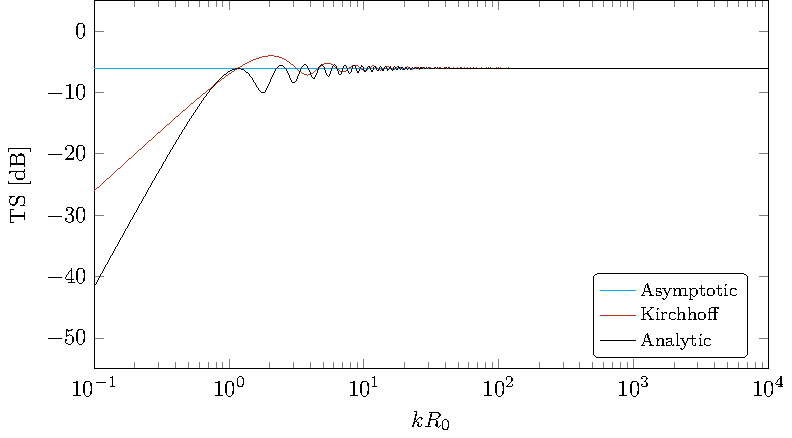
\includegraphics[width=\textwidth]{S1_3}
	\caption{\textbf{Scattering on a rigid sphere}: Comparison of the target strength (\Cref{Eq4:TS}) for the Kirchhoff approximation (\Cref{Eq4:exactHelmholtz}), the asymptotic limit (\Cref{Eq4:asymptotic_p_0}) and the analytic solution (\Cref{Eq4:backscatteredSolution}).}
	\label{Fig4:comparisonRigidSphere}
\end{figure}
\begin{figure}
	\centering
	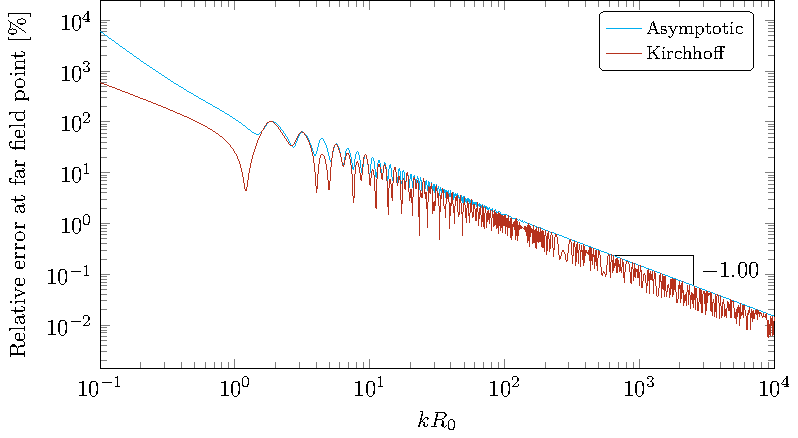
\includegraphics[width=\textwidth]{S1_4}
	\caption{\textbf{Scattering on a rigid sphere}: Comparison of the relative error for the far field backscattered pressure for the Kirchhoff approximation (\Cref{Eq4:exactHelmholtz}) and the asymptotic limit (\Cref{Eq4:asymptotic_p_0}) (compared to the analytic solution in \Cref{Eq4:backscatteredSolution}).}
	\label{Fig4:comparisonRigidSphereError}
\end{figure}


Consider a parametrization of the surface of a sphere given by
\begin{equation*}
	\vec{Y}(\xi,\eta) = R_0\begin{bmatrix}
		\cos\eta\cos\xi\\
		\cos\eta\sin\xi\\
		\sin\eta
	\end{bmatrix}
\end{equation*}
where $\xi\in(-\PI,\PI]$ and $\eta\in[-\PI/2,\PI/2]$. The surface element is then computed as
\begin{equation*}
	\idiff \Gamma(\vec{Y}) = \left|\pderiv{\vec{Y}}{\xi}\times\pderiv{\vec{Y}}{\eta}\right|\idiff\eta\idiff\xi = R_0^2\cos\eta\idiff\eta\idiff\xi
\end{equation*}
As the far field expression in \Cref{Eq4:monostatic} can be written as
\begin{align}\label{Eq4:integrandS1}
	p_0(\hat{\vec{x}}) &\approx -\frac{\imag kP_{\mathrm{inc}}}{2\PI}\int_{\Gamma_{\mathrm{i}}} \hat{\vec{x}}\cdot\vec{n}(\vec{y}) \euler^{-2\imag k \hat{\vec{x}}\cdot\vec{y}}\idiff \Gamma(\vec{y})\\
	&= -\frac{\imag kP_{\mathrm{inc}}R_0^2}{2\PI}\int_{\Gamma_{\mathrm{i}}}\hat{\vec{x}}\cdot\vec{n}(\vec{y}) \euler^{-2\imag k \hat{\vec{x}}\cdot\vec{y}}\cos\eta\idiff\eta\idiff\xi
\end{align}
we define the amplitude function $f$ by
\begin{equation*}
	f(\xi,\eta) = -\frac{\imag kP_{\mathrm{inc}}R_0}{2\PI}\hat{\vec{x}}\cdot\vec{Y}(\xi,\eta)\cos\eta
\end{equation*}
Moreover, let $g(\xi,\eta)$ be the oscillator function defined by
\begin{equation*}
	g(\xi,\eta) = \vec{d}\cdot \vec{Y}(\xi,\eta),\qquad \vec{d}=-2\hat{\vec{x}}.
\end{equation*}
The derivatives are found by
\begin{equation*}
\frac{\partial^{i+j}g}{\partial^i \xi \partial^j \eta} = \vec{d}\cdot \frac{\partial^{i+j}\vec{Y}}{\partial^i \xi \partial^j \eta}
\end{equation*}
Along the boundaries where $\eta=\pm\frac{\PI}{2}$ we have $\pderiv{g}{\xi} = 0$. That is, there are no oscillations at all (any point is a resonance point), and the numerical steepest descent cannot be used for the integral along these boundaries. However, as there are no oscillations, the integral can be computed with regular Gaussian quadrature.

Solving $\pderiv{g}{\xi}=0$ (for $\eta=\pm\frac{\PI}{2}$) yields solutions along $\tan\xi = \frac{d_2}{d_1}$ (for $d_1\neq 0$). If $d_1=0$ then solutions are found at $\xi=\pm\frac{\PI}{2}$ (for $d_2\neq 0$). For the case $d_1=d_2=0$, $\pderiv{g}{\xi}=0$ in the whole domain.

Solving $\pderiv{g}{\eta}=0$ yields solutions along $\cot\eta = \frac{d_1\cos\xi+d_2\sin\xi}{d_3}$ (for $d_3\neq 0$). If $d_3=0$ then solutions are found at $\eta=0$ and $\tan\xi=-\frac{d_1}{d_2}$ (for $d_2\neq 0$). For the case $d_2=d_3=0$, solutions are found at $\xi=\pm\frac{\PI}{2}$ and $\eta=0$.

Due to the periodicity, if $\nabla g(-\PI,\eta)=\zerovec$ for some $\eta$, then $\nabla g(\PI,\eta)=\zerovec$. Four boundary SPs ($\nabla g=0$) are found at 
\begin{equation*}
	(\xi,\eta) = \left(\arctan\left(-\frac{d_1}{d_2}\right),\pm\frac{\PI}{2}\right),\quad (\xi,\eta) = \left(\arctan\left(-\frac{d_1}{d_2}\right)-\sgn{-\frac{d_1}{d_2}}\PI,\pm\frac{\PI}{2}\right),
\end{equation*}
for $d_2\neq 0$, and at $(\xi,\eta) = (\pm\PI/2,\pm\PI/2)$ when $d_2=0$. Internal SPs are found at
\begin{equation*}
	(\xi,\eta) = \left(\arctan\left(\frac{d_2}{d_1}\right),\arccot\left(\frac{\sgn{d_1}\sqrt{d_1^2+d_2^2}}{d_3}\right)\right)
\end{equation*}
and
\begin{equation*}
	(\xi,\eta) = \left(\arctan\left(\frac{d_2}{d_1}\right)-\sgn{\frac{d_2}{d_1}}\PI,\arccot\left(-\frac{\sgn{d_1}\sqrt{d_1^2+d_2^2}}{d_3}\right)\right)
\end{equation*}
when $d_1\neq 0$ and $d_3\neq 0$. If $d_3=0$ and $d_1\neq 0$, SPs are found at 
\begin{equation*}
	(\xi,\eta) = \left(\arctan\left(\frac{d_2}{d_1}\right),0\right),\qquad (\xi,\eta) = \left(\arctan\left(\frac{d_2}{d_1}\right)-\sgn{\frac{d_2}{d_1}}\PI,0\right).
\end{equation*}
If $d_1=d_3=0$, SPs are found at $(\xi,\eta) = (\pm\PI/2, 0)$. If $d_1=0$ and $d_2\neq 0$
\begin{equation*}
	(\xi,\eta) = \left(\pm\frac{\PI}{2},\arctan\left(\pm\frac{d_3}{d_2}\right)\right).
\end{equation*}
There are no internal SPs for $d_1=d_2=0$.

The paths are found by inversion. If $\zeta=g(\xi,\eta)$ then
\begin{align*}
\eta = -\imag\Log\left(\frac{\frac{\zeta}{R}\pm\sqrt{\left(\frac{\zeta}{R}\right)^2-d_3^2-\gamma^2}}{\gamma-\imag d_3}\right)
\end{align*}
where $\gamma = d_1\cos\xi+d_2\sin\xi$. Correspondingly
\begin{equation*}
	\xi =-\imag\Log\left(\frac{\frac{\zeta}{R}-d_3\sin\eta\pm\sqrt{\left(\frac{\zeta}{R}-d_3\sin\eta\right)^2-\left(d_1^2+d_2^2\right)\cos^2\eta}}{(d_1-\imag d_2)\cos\eta}\right)
\end{equation*}
where it is assumed that $\cos\eta\not=0$ and $d_1-\imag d_2\not=0$ (in these cases there exist no inverse as $\pderiv{g}{\xi}=0$). The function $\Log$ is the principal valued natural logarithm defined by
\begin{equation*}
	\Log z= \ln|z|+\imag \Atan(y,x),\quad 
	\Atan(y,x) = \begin{cases}
	\arctan(\frac{y}{x}) & \mbox{if } x > 0\\
	\arctan(\frac{y}{x}) + \PI & \mbox{if } x < 0 \mbox{ and } y \ge 0\\
	\arctan(\frac{y}{x}) - \PI & \mbox{if } x < 0 \mbox{ and } y < 0\\
	\frac{\PI}{2} & \mbox{if } x = 0 \mbox{ and } y > 0\\
	-\frac{\PI}{2} & \mbox{if } x = 0 \mbox{ and } y < 0\\
	\text{undefined} & \mbox{if } x = 0 \mbox{ and } y = 0
	\end{cases}
\end{equation*}
for any non-zero complex number $z=x+\imag y$.

Consider the case of monostatic scattering from a unit sphere with $d_2=d_3=0$, $d_1=-2$, $R_0=\SI{1}{m}$ and $P_{\mathrm{inc}}=\SI{1}{Pa}$. Then the oscillatory function simplifies to
\begin{equation}\label{Eq4:simplified_g}
	g(\xi,\eta)=-2\cos\eta\cos\xi,
\end{equation}
and the amplitude function simplifies to
\begin{equation}\label{Eq4:simplified_f}
	f(\xi,\eta) = -\frac{\imag k}{2\PI}\cos\xi\cos^2\eta.
\end{equation}
Moreover, the paths for the integration in the $yx$-integration order is given by
\begin{align*}
v_\eta(\xi,q) = \arccos\left(\cos\eta-\frac{\imag q}{2\cos\xi}\right)
\end{align*}
and
\begin{equation*}
	u_\xi(p) = \arccos\left(\cos\xi-\frac{\imag p}{2\cos\eta_j}\right).
\end{equation*}
The paths for the integration in the $xy$-integration order is given by
\begin{equation*}
	u_\xi(p,\eta) = \arccos\left(\cos\xi-\frac{\imag p}{2\cos\eta}\right)
\end{equation*}
and
\begin{align*}
v_\eta(q) = \arccos\left(\cos\eta-\frac{\imag q}{2\cos\xi_i}\right).
\end{align*}
A quiver plot of the oscillatory function $g$ is given in \Cref{Fig4:quiver_g}, and the integrand (of equation \Cref{Eq4:integrandS1}) is visualized in the physical space and the parametric space in~\Cref{Fig4:rigidSphereCAD,Fig4:rigidSphereParm}, respectively.
\begin{figure}
	\centering
	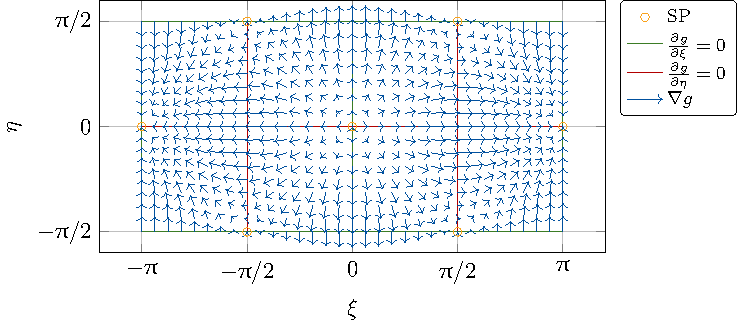
\includegraphics[width=0.8\textwidth]{S1_NSD_3}
	\caption{\textbf{Scattering on a rigid sphere}: Quiver plot of the gradient of $g(\xi,\eta)$ in \Cref{Eq4:simplified_g}. The stationary points (SPs) are marked by circles.}
	\label{Fig4:quiver_g}
\end{figure}
\begin{figure}
	\centering
	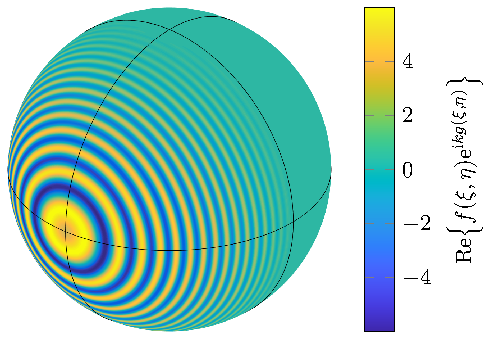
\includegraphics[width=0.6\textwidth]{S1_NSD_2}
	\caption{\textbf{Scattering on a rigid sphere}: The real part of the integrand (of equation \Cref{Eq4:integrandS1}) is visualized on a CAD model of a sphere with $kR_0=50$.}
	\label{Fig4:rigidSphereCAD}
\end{figure}
\begin{figure}
	\centering
	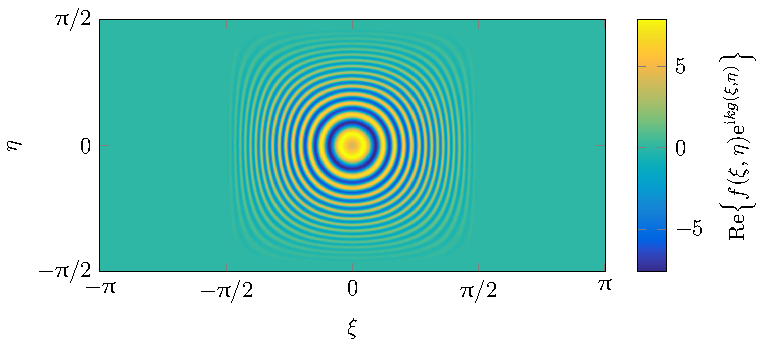
\includegraphics[width=0.8\textwidth]{S1_NSD_1}
	\caption{\textbf{Scattering on a rigid sphere}: The real part of the integrand (of equation \Cref{Eq4:integrandS1}) is visualized in the parametric space with $kR_0=50$.}
	\label{Fig4:rigidSphereParm}
\end{figure}

Due to symmetry it suffices to consider the domain $[0,\PI/2]^2$ (and multiply the results by four). The integrand over this domain is visualized in~\Cref{Fig4:rigidSphereParmSep}. In this domain we have stationary points in the origin and at the upper right corner $(\xi,\eta) = (\PI/2,\PI/2)$ (see~\Cref{Fig4:quiver_g}). Moreover, $\pderiv{g}{\xi}=0$ at the left and upper boundaries and $\pderiv{g}{\eta}=0$ at the right and lower boundaries. This yields an integrand around the top right corner which is significantly less oscillatory than the rest. The domain $\tilde{\Gamma}_1=[\PI/2-\delta,\PI/2-\delta]^2$ is for this reason, integrated with classical Gauss-Legendre quadrature. For convenience, define $\xi_1=0$, $\xi_2=\PI/2-\delta$, $\xi_3=\PI/2$, $\eta_1=0$, $\eta_2=\PI/2-\delta$, and $\eta_3=\PI/2$. The integral over $\tilde{\Gamma}_1$ may then be written as
\begin{equation*}
	I_{\mathrm{ne}} = \int_{\xi_2}^{\xi_3}\int_{\eta_2}^{\eta_3} f(\xi,\eta)\euler^{\imag k g(\xi,\eta)}\idiff\eta\idiff \xi
\end{equation*}
The size of this domain, governed by $\delta$, should be frequency dependent such that the number of needed quadrature points can remain fixed for all frequencies. 


Consider now the left domain $\tilde{\Gamma}_2=[0,\PI/2-\delta]\times [0,\PI/2]$. The integral over this domain may be decomposed as
\begin{align*}
	I_{\mathrm{w}} &= \int_{\xi_1}^{\xi_2}\int_{\eta_1}^{\eta_3} f(\xi,\eta)\euler^{\imag k g(\xi,\eta)}\idiff\eta\idiff \xi\\
	&=\int_{\xi_1}^{\xi_2}\left[\euler^{\imag k g(\xi,\eta_1)}\int_0^\infty f(\xi,v_{\eta_1}(\xi,q))\euler^{-k q}\pderiv{v_{\eta_1}}{q}(\xi,q)\idiff q\right.\\
	&{\hskip4em\relax}\left. -\euler^{\imag k g(\xi,\eta_3)}\int_0^\infty f(\xi,v_{\eta_3}(\xi,q))\euler^{-k q}\pderiv{v_{\eta_3}}{q}(\xi,q)\idiff q\right]\idiff \xi
\end{align*}
As $g(\xi,\eta_3)=0$ the latter integral over $\xi$ is not oscillatory and classical quadrature may be used to integrate over the variable $\xi$. On the other hand, the first integral over $\xi$ is oscillatory and we may use another decomposition to obtain the following
\begin{align*}
	I_{\mathrm{w}} = F_{\mathrm{yx}}(\xi_1,\eta_1) - F_{\mathrm{yx}}(\xi_2,\eta_1) -G_{\mathrm{yx}}(\eta_3)
\end{align*}
with $F_{\mathrm{yx}}$ as defined in~\Cref{Eq4:F_yx} and 
\begin{equation*}
	G_{\mathrm{yx}}(\eta) = \int_{\xi_1}^{\xi_2}\int_0^\infty f(\xi,v_{\eta}(\xi,q))\euler^{-k q}\pderiv{v_{\eta}}{q}(\xi,q)\idiff q\idiff \xi.
\end{equation*}
For the final integral over the domain $\tilde{\Gamma}_3=[\PI/2-\delta,\PI/2]\times [0,\PI/2-\delta]$ we integrate first over $\xi$ 
\begin{align*}
	I_{\mathrm{w}} &= \int_{\eta_1}^{\eta_2}\int_{\xi_2}^{\xi_3} f(\xi,\eta)\euler^{\imag k g(\xi,\eta)}\idiff\xi\idiff \eta\\
	&=\int_{\eta_1}^{\eta_2}\left[\euler^{\imag k g(\xi_2,\eta)}\int_0^\infty f(u_{\xi_2}(p,\eta),\eta)\euler^{-k q}\pderiv{v_{\eta_1}}{q}(\xi,q)\idiff q\right.\\
	&{\hskip4em\relax}\left. -\euler^{\imag k g(\xi_3,\eta)}\int_0^\infty f(u_{\xi_3}(p,\eta),\eta)\euler^{-k q}\pderiv{v_{\eta_m}}{q}(\xi,q)\idiff q\right]\idiff \eta.
\end{align*}
The latter integral over $\eta$ is again not oscillatory since $g(\xi_3,\eta)=0$ and classical quadrature may be used here. The first integral over $\eta$ is oscillatory and we may use another decomposition to obtain the following
\begin{align*}
	I_{\mathrm{se}} = F_{\mathrm{xy}}(\xi_2,\eta_1) - F_{\mathrm{xy}}(\xi_2,\eta_2) -G_{\mathrm{xy}}(\xi_3)
\end{align*}
with $F_{\mathrm{xy}}$ as defined in~\Cref{Eq4:F_xy} and 
\begin{equation*}
	G_{\mathrm{xy}}(\xi) = \int_{\eta_1}^{\eta_2}\int_0^\infty f(u_{\xi}(p,\eta),\eta)\euler^{-k p}\pderiv{u_{\xi}}{p}(p,\eta)\idiff p\idiff \eta.
\end{equation*}
Summing up each contribution yields the far field monostatic pressure
\begin{equation*}
	p(\hat{\vec{x}}) = 4(I_{\mathrm{ne}}+I_{\mathrm{w}}+I_{\mathrm{se}})
\end{equation*}
\begin{figure}
	\centering
	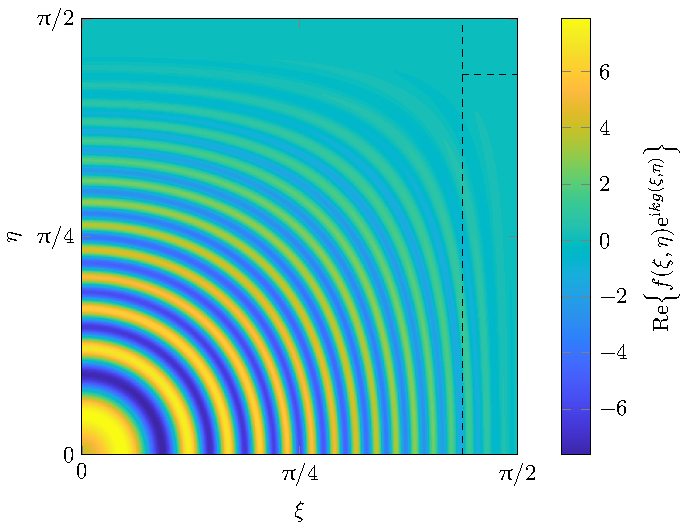
\includegraphics[width=0.8\textwidth]{S1_NSD_8}
	\caption{\textbf{Scattering on a rigid sphere}: The integration domain over $[0,\PI/2]^2$ is separated into three parts separated by the dashed lines.}
	\label{Fig4:rigidSphereParmSep}
\end{figure}

In \Cref{Fig4:polygonApproxTS,Fig4:polygonApproxError} some results of Kirchhoff approximation using polygonal approximation of the geometry in \Cref{Eq4:polygonalApprox} are presented. We here use the triangulation method based on the exact CAD model in \Cref{Fig4:SphericalShellCAD} described in the introduction. The key observation is that the error is not only depending on the geometrical approximation, but also the frequency resolution of the problem which is consistent with the results presented in \cite{Fillinger2014aen} and discussed in \cite{Gilroy2017tes}. From \Cref{Fig4:polygonApproxError}, we can deduce experimentally that the relative error for the polygonal approximation of the Kirchhoff approximation goes as $E_{\mathrm{r}}\sim 14h^2kR_0$ for high frequencies. This contradicts the claim made in \cite{Schneider2003asb} and \cite{Oestberg2016tes} that the size limitation of the triangle only depends on the approximation of the curvature of the object. However, the number of points is greatly reduced compared to using classical Gaussian quadrature on the exact geometry.
\begin{figure}
	\centering
	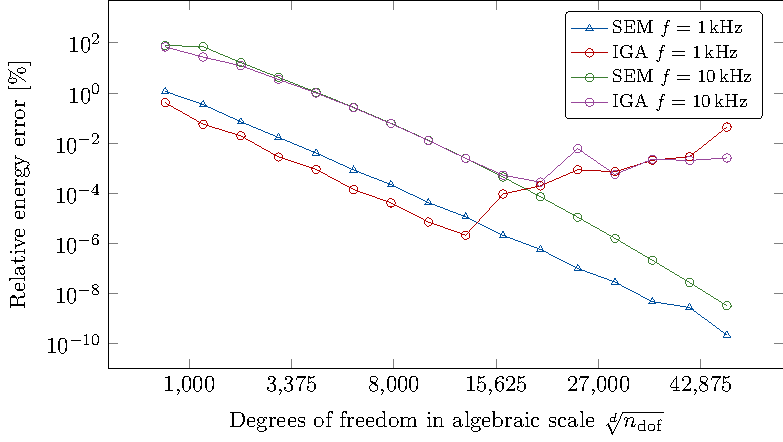
\includegraphics[width=\textwidth]{S1}
	\caption{\textbf{Scattering on a rigid sphere}: Comparison of Kirchhoff approximation using a polygonal approximation of the geometry (\Cref{Eq4:polygonalApprox}) instead of exact geometric representation by NURBS. The exact Kirchhoff approximation is given by \Cref{Eq4:exactHelmholtz}.}
	\label{Fig4:polygonApproxTS}
\end{figure}
\begin{figure}
	\centering
	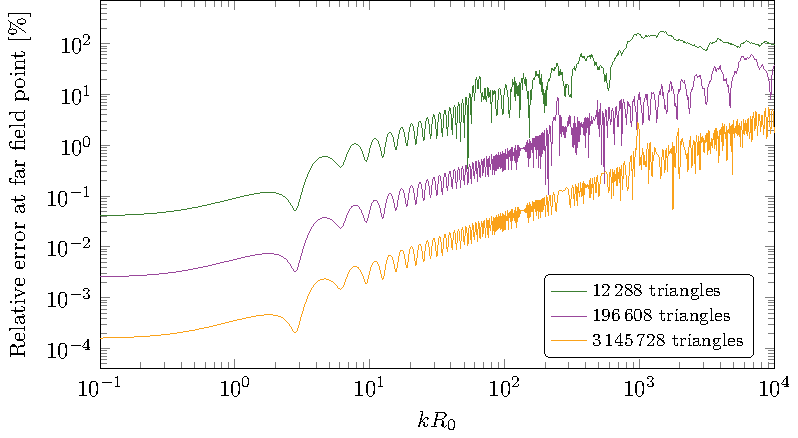
\includegraphics[width=\textwidth]{S1_2}
	\caption{\textbf{Scattering on a rigid sphere}: Comparison of Kirchhoff approximation using a polygonal approximation of the geometry (\Cref{Eq4:polygonalApprox}). The reference solution is the exact Kirchhoff approximation in \Cref{Eq4:exactHelmholtz}.}
	\label{Fig4:polygonApproxError}
\end{figure}


For the hybrid NSD consider a rather large size of the domain $\tilde{\Gamma}_1$ (compared to the frequency) given by ${\delta = \min\{\PI/2,9/\sqrt{k}\}}$ (heuristically obtained). The Gauss-Legendre integrals are evaluated by a (fixed) $100^{\mathrm{th}}$ order quadrature scheme. The integrals for the numerical steepest descent are computed by a $5^{\mathrm{th}}$ order Gauss-Laguerre quadrature scheme. Whenever the oscillatory integrals span less than 5 wavelengths Gauss-Legendre integration is used. For this reason, we call the method a hybrid numerical steepest descent.

As expected, and illustrated in \Cref{Fig4:gaussVSnsd}, using classical Gauss-Legendre quadrature to approximate the integrals in the Kirchhoff approximation yields poor results for higher frequencies. Combining Gauss-Legendre quadratures with the numerical steepest descent into the hybrid method resolves the problem for higher frequencies. This hybrid method will converge for all frequencies as opposed to the triangular approximation approach as illustrated in \Cref{Fig4:gaussVSnsd2}.

\begin{figure}
	\centering
	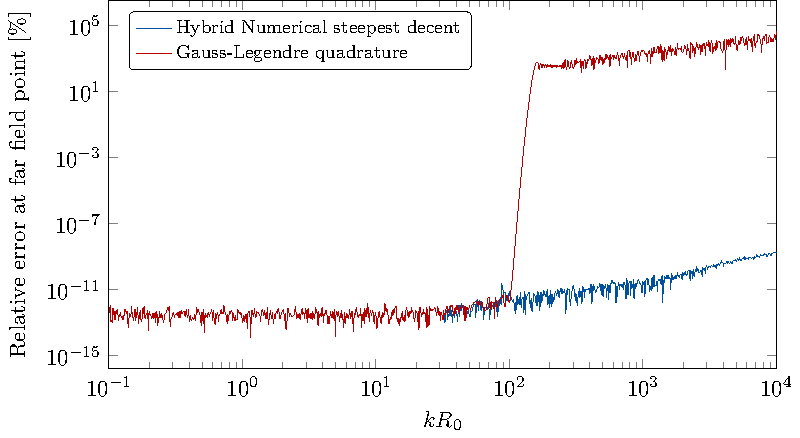
\includegraphics[width=\textwidth]{S1_NSD_6}
	\caption{\textbf{Scattering on a rigid sphere}: Comparison of Kirchhoff approximation using standard Gauss-Legendre quadrature and using numerical steepest descent. The reference solution is the exact Kirchhoff approximation in \Cref{Eq4:exactHelmholtz}.}
	\label{Fig4:gaussVSnsd}
\end{figure}
\begin{figure}
	\centering
	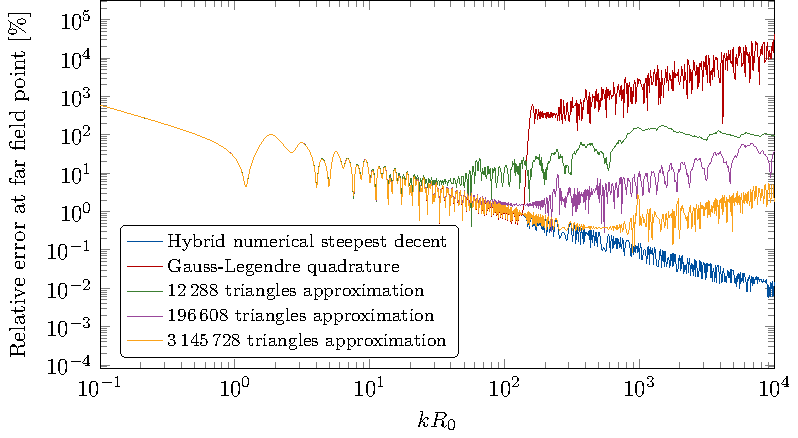
\includegraphics[width=\textwidth]{S1_NSD_7}
	\caption{\textbf{Scattering on a rigid sphere}: Comparison of Kirchhoff approximation using standard Gauss-Legendre quadrature and using numerical steepest descent, in addition to the polygon approximation of the geometry. The reference solution is the analytic solution in \Cref{Eq4:backscatteredSolution}.}
	\label{Fig4:gaussVSnsd2}
\end{figure}

The computational savings for the hybrid NSD method compared to the triangularized approach is significant. For example, to achieve engineering precision (\textless 1\%) accuracy for $kR_0=10^3$ we can see from~\Cref{Fig4:polygonApproxError} that the triangularized approach needs about \num{3e6} triangles. This single simulation is computed in roughly 160 second whereas the numerical steepest decent only need about 1 second (and obtaining machine epsilon precision). It is much easier to implement an efficient triangularized formulation than the NSD formulation, and so we would like to argue that the computational savings of using the NSD formulation could potentially be even greater.